\subsection*{(iii)}

A simulation of the account is provided below.

\begin{figure}[h]
    \centering
    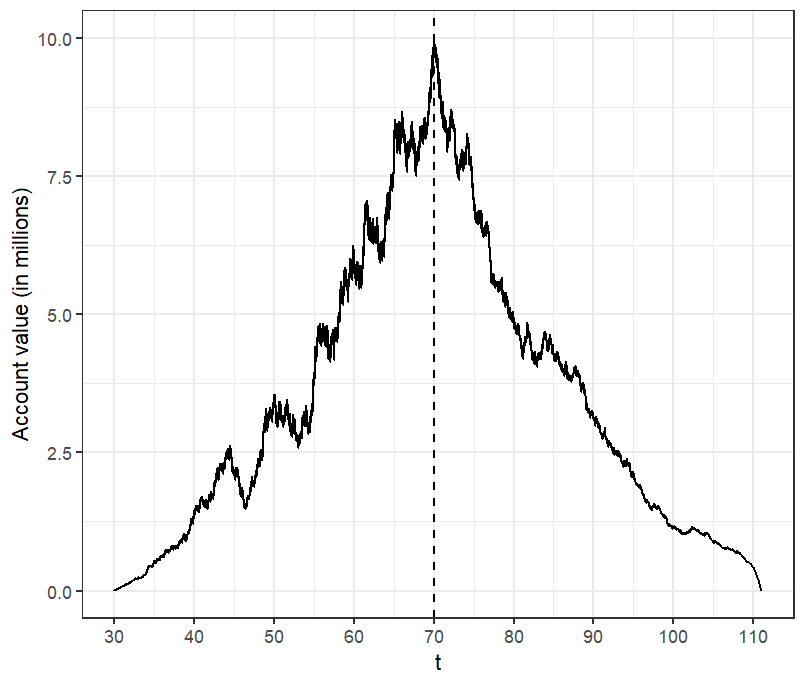
\includegraphics[width=0.5\linewidth]{Pictures/SimulationOfAccountPath.png}
\end{figure}

We observe from our simulation that it begins from age $t=30$ at the value of zero as demanded. Thereafter, the account accumulates until retirement $m = 70$ with a value of around 9.8 million (monetary units). Then the account de-cumulates until our assumed lifetime cut-off at $t = 111$. We also observe random fluctuates due to the fact that we model the risky asset via a Brownian motion.